%----------------------------------------------------------------------------
\chapter{Előismeretek}\label{sect:Preliminaries}
%----------------------------------------------------------------------------
\section{Essbase adatbázis}
Alapvetően kétféle adatbázis típus létezik lekérdezés szempontjából. Az egyik az OLTP (On Line Transaction Processing, online tranzakciófeldolgozás), ahol sok tranzakció van és ezek kis módosításokat (UPDATE,INSERT), vagy kisebb, rövidebb ideig tartó lekérdezéseket végeznek el az adatbázisban. A másik az OLAP (On Line Analitical Processing vagy online analitikai feldolgozás), ami kimondottan a lekérdezésekre lett optimalizálva, jelentések készítésére. Ilyen adatbázis például az Essbase.

OLAP Kocka:     Az elemezni kívánt dimenziók szintjei és hierarchiája alapján összevont értékeket tároló adatszerkezet. A kockák sokféle dimenziót – időt, földrajzi helyet stb. – képesek összekapcsolni különböző összesített adatokkal – például a gépjárműveket a szervezeti egységekkel. A kockák nem a szigorúan vett matematikai értelemben kockák, mivel nem biztos, hogy egyenlők az oldalaik. Ennek ellenére egy nagyon szemléletes metaforái egy bonyolult koncepciónak. Az Essbase adatbázis OLAP kockák összességéből áll.

Érték: A kockákban lévő értékek, amelyek a kocka ténytáblájának valamely oszlopán alapulnak, és általában numerikus értékek. A mértékek a kocka központi értékei – előfeldolgozhatók, aggregálhatók és elemezhetők. A mértékekre gyakori példa a forgalom, a profit, a bevétel és a költség. Egy mérték a kocka összes lekötött dimenziójából adódik. Például meg kell adni milyen év, melyik szervezeti egység, melyik konkrét autó stb.

Tag: Azok az attribútumok, amikhez értékek kötődnek, például egy konkrét gépjármű.

Csoport: Valamennyi tagok összessége.

Dimenzió: A szintek szervezett hierarchiáinak együttese egy kockában, amit a felhasználó megért, és az adatelemzés alapjaként használ. A földrajzi hely dimenziója például tartalmazhatja az ország, a megye és a város szinteket. Az idő dimenziója pedig tartalmazhatja az év, a negyedév, a hónap és a nap szintet. A kimutatásokban és kimutatásdiagramokban minden hierarchia mezőegyüttessé válik, amelyek kibonthatók és becsukhatók az alacsonyabb és magasabb szintek felfedése érdekében.

Hierarchia: A kocka megjelenítése két dimenzióban.

\pagebreak

 \begin{figure}[!ht]
\centering
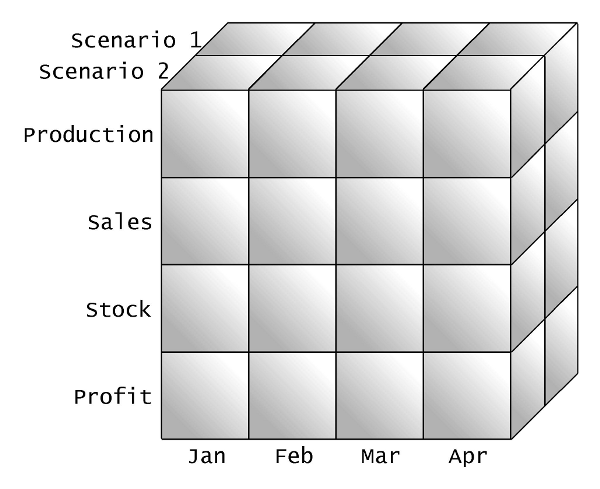
\includegraphics[width=80mm, keepaspectratio]{figures/cube1.png}
\caption{Példa kocka} 
\label{fig:Cube1}
\end{figure}

 \begin{figure}[!ht]
\centering
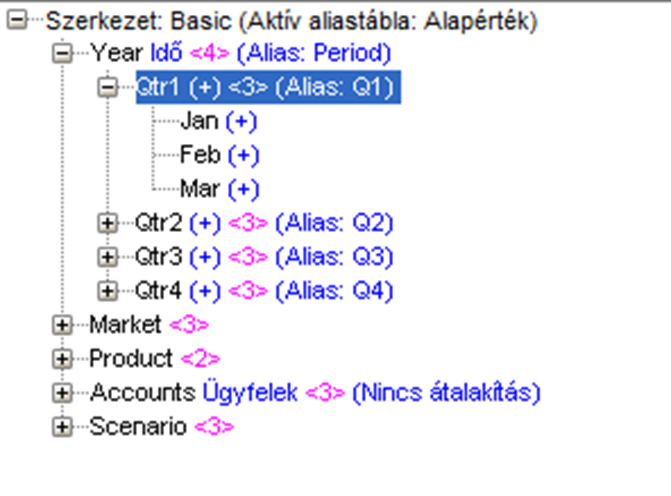
\includegraphics[width=100mm, keepaspectratio]{figures/hierarchy.png}
\caption{Példa Hierarchia} 
\label{fig:Cube1}
\end{figure}


\subsection{Essbase lekérdezések}

Essbase-ből alapvetően kétféle képpen lehet lekérdezni, riportban és mdx-ben. A riport lekérdező nyelv tipikusan kimutatásokhoz használható jól, ha valamit összevontan szeretnénk lekérdezni a kockából. Ezzel szemben az MDX egy standard lekérdező nyelv, amibe egyrészt lehet sql szerű lekérdezéseket írni, másrészt adatmódosító műveleteket is lehet használni. Ilyen adatmódosító művelet például az Allocation parancs, ahol egy csoportból vagy  
\subsubsection{Riport}


\subsubsection{MDX}

\subsection{Essbase esettanulmány}
Tegyük fel, hogy van egy céges autónk és szeretnénk eltárolni az autó forgalmi adatait, hová ment, közbe mennyi volt a fogyasztása. Ezt tipikusan OLTP adatbázisba érdemes tárolni, mert sok tranzakció keletkezik, sok beszúrás művelettel. Ellenben tegyük fel, hogy több céges autónk van és az autókra keletkeznek kölségek, például benzin, amortizáció. Valamint tételezzük föl hogy ezekből a költségekből van olyan, ami az egész szervezeti egységhez kötődik, például a benzint egyszerre vesszük meg és mindenki tankol ebből annyit amennyire szüksége van. Ezek a költségek az OLTP adatbázisunkba vannak eltárolva egy táblába autókra és szervezeti egységekre külön. Ha megvannak ezek az adataink, akkor gyakran felmerülő igény, hogy le szeretnénk kérdezni valamilyen szempont szerint aggregálva ezeket a költségeket. Például összeadni vagy átlagolni hogy egy autóra és szervezeti egységre mennyi költség keletkezett. Egy ilyen lekérdezés, nagy tábla esetén sokáig tart, mert a tábla összes során végig kell menni.  Ebben az esetben már érdemes felépíteni egy OLAP kockát, erre az OLTP adatbázisra, ami automatikusan képes az ilyen jellegű aggregációra, összeadásra, átlagolásra stb. Ezen kívűl képes arra is, hogyha keletkezik olyan költség ami egy szervezeti egységhez köthető (az előzőekben említett benzin amit egyszerre veszünk), azt le tudja osztani minden egyes autóra lebontva, például megtett út alapján.

\section{Xtext keretrendszer}
Az Xtext egy olyan keretrendszer, amiben saját szakterület specifikus programozási nyelvet lehet definiálni. Ha ez kész, akkor ebben a programozás nyelvben lehet utána fejleszteni, majd ezt a kódot az Xtext tudja validálni és feldolgozni, ezeket az adatokat objekumokba megkapjuk és java-ban ezt utána fel lehet dolgozni.

\section{Eclipse plugin}
Az Eclipse fejlesztő környezet egy modulokkal (úgynevezett pluginekkel) bővíthető keretrendszer, melyek segítségével saját funkciókkal szabhatjuk testre a környezetet. Önálló laboratórium során, én is készítek egy saját plugint, szerkesztőt, amibe a létrehozott programozási nyelv kódját lehet szerkeszteni.

\section{Latex és riportolási technikák}
Megjelenítésre, riport kimenetnek a dolgozatomban én latexet választottam, mert a forráskódja java kódból generálható és vannak olyan grafikus megjelenítő csomagjai, amivel az Essbase-ből kijövő nyers adatokat meg lehet jeleníteni.

\section{Xtend}
Sok új nyelvi elemmel rendelkező java nyelv továbbfejlesztése. Hasznos funkciója, hogy lehet olyan szöveg sablont készíteni, amiből az Xtend java osztályokat generál StringBuilder-ek segítségével és egyszerű paraméterezéssel meg lehet adni a sablonnak a változó értékeket.

